\section{Introduction}
The spherical shallow water equations serve as an effective test bed for 
assessing numerical methods for general circulation models (GCMs). They 
exhibit many of the dynamics and complexities of the full 3D equations with 
the advantage of being two-dimensional and computationally less intensive.  
Full 3D models combine the dynamical core of the GCM with
 a plethora of sub-grid parameterizations 
schemes for unresolved physical and thermodynamical processes further 
adding to their complexity.  However, shallow water type models and 
the unforced test cases traditionally associated with them \citep{Williamson:1992kx}
are missing key features (e.g. water vapor, convection, latent heat release, 
thermal forcing) which play key roles in atmospheric and 
climatological phenomena. Including simplified forcing mechanisms to represent 
such moisture and heating
processes in the shallow 
water system narrows the gap between idealized unforced studies 
and full-physics models can be bridged. These forced shallow water 
models include the dynamical complexities of the full models and can retain
the non-linearity of the physical processes.  However,
the shallow water equations are still simple enough to effectively study
the key components of the dynamical core like the numerical alogrthims,
computational grid, and for variable resolution and AMR models, grid refinement
strategies and effectiveness. Shallow water models have the added advantage of 
being computationally cheap and efficient to run at high resolutions.

A variety of studies have implemented forcing in shallow water models to study
 the fundamental dynamical aspects of large synoptic
scale climatological features such as the Madden-Julean Oscillation (MJO)
and intense, small scale features such as tropical cyclone 
evolution, cumulus convection, and frontal propagation.
\cite{ferreira1996dynamical} and \cite{yang2013triggered} implement
spatial and temporal varying mass sinks and sources within nonlinear 
shallow-water models to simulate MJO convection in studies of MJO
induced twin tropical cyclones and MJO's convective envelope 
development, respectively. In \cite{enagonio2001tropical}, 
the authors examined tropical cyclogenesis
by forcing a shallow water system with periodic pulses of vorticity  to represent multi-burst convection.
 \cite{hendricks2014hurricane} mimicked diabatic heating in hurricane 
eyewalls in a cartesian shallow water model by using a prescribed annular,
 axisymmetric mass sink.

A framework to specifically study the dynamical role of moist processes in a shallow water system
was proposed in the seminal work by \cite{gill1982studies}. In this system
 a moisture equation with nonlinear precipitation thresholds was added to the 
linearized shallow-water equations to model the effects of latent heat release on the 
propagation of large scale disturbances. Similar models incorporating this framework for 
parameterizing moisture were analyzed by \cite{goswami1991modification} to study
large-scale equatorial waves propagation and by \cite{frierson2004large},
\cite{stechmann2006structure}, and \cite{bouchut2009fronts} in the context of tropical precipitation 
fronts. Unlike the others, \cite{bouchut2009fronts} implements the moist-convective 
parameterizations in a fully nonlinear rotating shallow water model,
which \cite{lambaerts2011moist} also used to compare the difference in the evolution 
of barotropic instability between moist and dry conditions. To study the
dynamical role of moisture in tropical cyclone instabilities, \cite{lahaye2016understanding} 
used this moist rotating shallow-water model with the addition of an evaporation 
mechanism. \cite{rostami2017influence} implemented both a 1-level barotropic 
version and a 2-level shallow water baroclinic version of the model introduced in 
\cite{lambaerts2011moist} to study large-scale small Rossby number vortices.

Other frameworks for simulating precipitation and convection in the shallow water
system that have been implemented recently included models by 
\cite{wursch2014simple} and \cite{zerroukat2015moist}.
\cite{wursch2014simple} developed a simplified model of cumulus convection 
incorporating representation of updrafts, downdrafts and idealized precipitation 
effects, in a 1D shallow water model. 
Once, the fluid exceeds a certain threshold height, signaling the 
onset of convection and mechanisms that serve as a simplified representation 
of cumulus convection kick by modifying the geopotential height to creates 
conditional instability mimic updrafts. 
This method was extend to a rotating, two dimensional shallow 
water model in \cite{kent2017dynamics}.
In \cite{zerroukat2015moist}, the authors re-derived the two-dimensional
shallow water system from the three-dimensional moist Boussinesq 
approximation. Density was permitted to very with temperature which
resulted in addition buoyancy related terms in the momentum equations
permitting a dynamics moisture feedback. \cite{zerroukat2015moist} also 
implements a three-state moisture model consisting of vapor, cloud, and 
precipitated species.

In this paper, we implement two forcing frameworks that seek to mimic moisture 
and convection in a spherical, 2d shallow water system. In the first framework, 
a moist shallow water equations derived in \cite{bouchut2009fronts} and 
\cite{lahaye2016understanding} precipitation causes
 convective forcing cause tropical-cyclone like vortices to develop and strengthen. In the second 
framework, the barotropic instability shallow water test case of 
\cite{galewsky2004initial} is implemented within a different moist shallow water system developed from 
 \cite{zerroukat2015moist}. As the jet becomes unstable and collapses, front like 
 systems with clouds and precipitation develop. Using these frameworks, we
 investigate the distinctive dynamics produced by the non-linear physics processes
 within the traditional shallow water system. A main goal of this paper is to
 introduce test cases with more challenging complex and transient features
 to specifically test the ability of adaptive mesh refinement (AMR) 
 to track and resolve these moving and growing features.
 
 We utilize 2D shallow water 
 version of the fourth-order cubed-sphere finite-volume AMR model
 presented in \cite{mccorquodale2015adaptive} and
 \cite{ferguson2016analyzing}. The model implements dynamic refinement using
 a mapped-multiblock AMR technique that overlays the base grid with refined patches.
 Using AMR, we observe how features in the test cases evolve due to the forcing 
 processes and how those forcing processes are affected by the AMR refinement. 
Ideally the physics forcing schemes should be able to effective span 
the multiple levels of refinement and changing resolutions created by AMR.
 In addition, we seek to quantify improvements gained from AMR grids
 and determine effective refinement criteria.

This chapter is organized as follows. Section 2 provides a brief overview
of the finite volume model and the Chombo multiblock AMR techniques.
Section 3 describes the setup for the shallow water equations
with moist convective forcing and the strengthening vortex test case.
Section 4 compares numerical results of the strengthening vortex
test case for uniform and AMR runs of varying resolution. The
 \cite{zerroukat2015moist} moist shallow water system's use with
 the barotropic instability test case and its numerical results
 are presented in Section 5.  Section 6 summarizes our
 conclusions from the two test cases.

\section{High-Order Finite-Volum Chombo AMR Model}
  For this study we employ an unstaggered finite-volume (FV) mapped-multiblock dynamical core (dycore) that is fourth-order accurate and adaptive in both space and time. The model's adaptive mesh refinement is based on the Chombo AMR library \citep{Adams:2015gd}, and a in-depth description of the model setup for the shallow-water equations on an equiangular cubed-sphere grid can be found in \cite{mccorquodale2015adaptive}. The model is mass conserving and conserves energy up to the temporal truncation error, when limiters or explicit dissipation are not applied. 
  
  The cubed-sphere grid consists of a cube whose six separate panels are `deflated' onto the surface of a sphere. In addition to eliminating the polar singularities found in spherical latitude-longitude grids, the equiangular cubed-sphere also leads to a quasi-uniform mesh with similarly sized grid cells across the sphere. The discrete resolution of the cubed-sphere grid is denoted by $c\{N_c\}$ where $N_c$ is the number of grid cells in each direction on a panel. Several properties of the equiangular cubed-sphere grid, including approximate grid spacings, are given in Table~\ref{tb:grids} for resolutions used in this paper. 

\begin{table}[t]
    \caption{Properties for several cubed-sphere grid resolutions where 
    $N_c$ is the number of cells along an edge of a cubed-sphere panel.
    Here the number of cells is the total number of grid cells 
    ($N_c^2 \times 6$), $\Delta x$ is the approximate grid spacing, 
    $A_{avg}$ is the average area of a grid cell, $A_{min}/A_{max}$ is the
    ratio between the minimum and maximum cell areas, Eq.  Res.  is the
    grid resolution in degrees given by $90^\circ / N_c$, and $RLL_{equiv}$
    is the equivalent grid spacing on a regular latitude-longitude
    grid with the same total number of cells.}%
    \label{tb:grids}
    \begin{center}
    \begin{tabular}{cccrccc}
            \hline
            Resolution ($N_c$) & No. of cells       & $\Delta x$ (km) & $A_{avg} (\mbox{ km}^2)$ & $A_{min}/A_{max}$ & Eq. Res.     & $RLL_{equiv}$ \\ 
            \hline
            \hline
            c$32$              & $6.14 \times 10^3$ & $313$           & $8.302 \times 10^{4}$    & $0.7249$          & $2.81^\circ$ & $3.25^\circ$  \\ 
            c$64$              & $2.46 \times 10^4$ & $156$           & $2.076 \times 10^{4}$    & $0.7159$          & $1.41^\circ$ & $1.62^\circ$  \\ 
            c$128$             & $9.83 \times 10^4$ & $78.2$          & $5.189 \times 10^{3}$    & $0.7115$          & $0.70^\circ$ & $0.82^\circ$  \\ 
            c$256$             & $3.93 \times 10^5$ & $39.1$          & $1.297 \times 10^{3}$    & $0.7093$          & $0.35^\circ$ & $0.41^\circ$  \\ 
            c$512$             & $1.57 \times 10^6$ & $19.5$          & $3.243 \times 10^{2}$    & $0.7082$          & $0.18^\circ$ & $0.20^\circ$  \\ 
            c$1024$           & $6.29 \times 10^6$ & $9.77$          & $8.107 \times 10^{1}$    & $0.7076$          & $0.09^\circ$ & $0.10^\circ$  \\ 
            c$2048$           & $2.52 \times 10^7$ & $4.89$          & $2.027 \times 10^{1}$   & $0.7074$          & $0.04^\circ$ & $0.05^\circ$ \\
            \hline
        \end{tabular}
    \end{center}
\end{table}
  
  The model uses a classical fourth-order Runge-Kutta (RK4) time discretization scheme. The model's finite-volume spatial discretization implements a fourth-order accurate discretization to compute flux averages on the faces and a high-order least-squares interpolation to compute stencil operations near panel or block boundaries. The stencil operations are used to create three layers of ghost cells at the panel edges to preserve the order of accuracy of the fluxes. At a panel edge, the fluxes for cell faces that lie on the panel edge are calculated separately for each panel and then averaged together. The mean value is then taken as the flux for each face to ensure conservation. Additionally, a sixth-order diffusive operator is applied to smooth the flux calculations while still maintaining the scheme's fourth-order accuracy. 
  
  The only communication between the computational domains for each panel are the cell values needed to interpolate the ghost cells and the face fluxes at the domain edge. The AMR multiblock method used permits further subdivision of the panel domains into rectangular sections of grid cells, called patches. The communication between patches domains is similarly limited as for panel domains. This structure permits the numerical calculations to be distributed efficiently across many processors on large parallel computer systems.
  
  The model's mapped multiblock AMR approach implements a hierarchy of nested grid levels of increasing resolution, using the numerical tools developed in the Chombo AMR library \citep{Adams:2015gd}. The higher resolution grid levels, which have a defined refinement ratio with the coarser levels, are overlaid on top of the coarser levels. Finer levels are placed over regions where coarse cells have been marked (tagged) by the model as meeting the refinement criterion. The cells values in the finer level are initialized via interpolations from the coarser level. Ghost cells are used to calculated the fluxes at the level boundaries in the same manner as is done at the cubed-sphere panel boundaries. If multiple levels are used, intermediate levels must cover enough area to ensure that the finer level is proper nested to ensure that the ghost cells for the finer level are interpolated from cells only on the intermediate level.  
  
  Finer levels are sub-cycled in time to maintain a constant Courant number across all resolutions. The sub-cycling routine can be summarized as follows. After interpolating values to the refined level, the coarser level is advanced a time step. The finer level is then advanced in time using a finer time step determined by dividing the coarse time step by the refinement ratio between the two levels.  At each finer time step the ghost cells used to calculate the boundary fluxes at the finer level's edges are updated via a temporal interpolation from the RK4 method. After the sub-cycling is complete, the values on the coarse grid is updated from the solution on the finer grid.  \cite{mccorquodale2015adaptive} and \cite{ferguson2016analyzing} both provide more detailed descriptions of the AMR technique. 
  
  The refinement criteria that determine over which regions additional gird levels are placed are based on user-selected threshold values for flow properties.  The thresholds are set independently for each simulation and the criteria can be based on a variety of properties such as tracer values, gradients, relative vorticity, or a combination of multiple properties.  The AMR dycore is can have multiple levels of refinement, preset for each simulation, and tagging criteria can be uniform across all levels or they can scale with increasing resolution.
 
%--------Section 
\section{Fake Tropical Cyclones} 
  This test cases simulates the growth and development of tropical cyclone-like 
  vortices in a 2D shallow water framework using a moist convective forcing 
  mechanism. Weak vortices are initialized on a calm and uniform height 
  background field. Evaporation and precipitation cause the vortices to strengthen. 
  After several days of strengthening the orderly vortices collapse and a more chaotic 
  system evolves with several small vortices and jet-like background flow developing. 

  We first provide a description of the moist convective shallow water system 
  and an overview of the initial conditions. Next We present the evolution of an 
  isolated vortex in this test case at a uniform high resolution. Then we demonstrate
  the use of AMR in this test case comparing the affects of different resolutions and
  various tagging criteria.

%Subsection
  \subsection{``Moist-convective`` shallow water equations }
     The shallow water equations are modified to include the transport of a 
     moisture variable and the effects of moist convection, precipitation, and evaporation. 
     We extend to the generalized 2D shallow water equations for the sphere the framework
     of a rotating shallow water model that includes precipitation and convection 
     presented in \cite{bouchut2009fronts} and \cite{lahaye2016understanding}, 
     which added evaporation. The rotating shallow water version of this scheme 
     has been used to study the combined effects of precipitation, latent heat release, 
     and the nonlinearity of the primitive equations 
     (\cite{bouchut2009fronts},\cite{lambaerts2011moist}, \cite{lahaye2016understanding}).
     
     In this moist convective system, a relaxation sink is added to the moisture equation (Eq. \ref{eq:swqcon}), 
     representing precipitation for when moisture levels exceed a saturation value. 
     A corresponding convective mass sink is added to the continuity equations. A 
     moisture source is added to the moisture equation to represent evaporation. 
     The equations for this modified shallow water system are
   \begin{equation}
     \label{eq:swmom} \frac{\partial h \mathbf{v}}{\partial t} +
     \nabla \cdot ( h \mathbf{v} \mathbf{v}) + f \mathbf{\hat{k}}\times(h\mathbf{v}) + gh\nabla H = 0
   \end{equation}
   \begin{equation}
     \label{eq:swcon}  \frac{\partial h}{\partial t} + \nabla \cdot (h\mathbf{v}) = - \beta P 
   \end{equation}
   \begin{equation}
     \label{eq:swqcon}  \frac{\partial hQ}{\partial t} + \nabla \cdot (hQ\mathbf{v}) = h(E - P).
   \end{equation}
   Here $\mathbf{v}$ is the velocity vector, $\mathbf{v}\mathbf{v}$ denotes the outer product
   of the velocity vector, $f$ is the Coriolis parameter, $g$ is 
   the acceleration due to gravity,
   $h$ is the height of the fluid, $H$ is the total height including topography, and 
   moisture variable $Q$ represents bulk humidity. 
   $E$ is the evaporation in the moisture budget and $P$ is the precipitation . 
   The latent heat release from precipitation does not directly influence the 
   horizontal momentum. Instead it is linked to convective vertical velocity 
   directly proportional to $P$ at the upper surface of the fluid.
   Since this system is designed to represent only the lower part of the 
   troposphere, the convective updraft can be constructed as a mass exchange 
   from this surface layer. The mass exchange is then represented as a mass 
   sink in Equation \ref{eq:swcon}, governed by an adjustable
   constant $\beta$.  A detailed explanation for the implementation is 
   presented by \cite{bouchut2009fronts}.

   The precipitation sink is calculated in terms of $Q$ and the saturation value $Q_s$,
   \begin{equation}
     \label{eq:precip} P = \frac{Q-Q_s}{\tau}\mathbf{H}(Q-Q_s).
   \end{equation}
   with a relaxation time of $\tau$. $\mathbf{H}(\cdot)$ is the Heaviside function
    so that $P = 0$ whenever $Q \leq Q_s$.
   For evaporation, a common parameterization used in \cite{lahaye2016understanding} is modified
   to include an upper velocity limit on the evaporation rate.  The evaporation source term is thus
   %\begin{equation}
     \begin{align}
        \label{eq:evap} 
     &E  =   \alpha_e  \lvert \vec{v} \rvert & \mathrm{for} \ \lvert \vec{v} \rvert < v_\mathrm{max} \nonumber \\
     &E  =   \alpha_e (v_\mathrm{max}) &  \mathrm{for} \ \lvert \vec{v} \rvert > v_\mathrm{max} 
     \end{align}
   %\end{equation} 
   where the evaporated moisture is dependent on the magnitude of the 
   velocity $\vec{v}$ and the adjustable coefficient $a_e$. Evaporation scales 
   with wind speed until $v_{\mathrm{max}}$. In the simulations presented below
   $a_e = 0.055$ and $v_{\mathrm{max}} = 30 \mathrm{m/s}$
   At higher velocity magnitudes, $E$ is constant.
   As established, evaporation is unlimited, but such a setup can lead to runaway 
   supersaturation and very large height forcing that causing exceedingly high wind 
   velocities and even negative height values in longer simulations.
    
    To limit these sources of instability, we implement additional mechanisms
    to the forcing mechanics. Evaporation moisture is drawn from a finite reservoir 
    $C_r(\phi,\lambda)$ so that $E$ cannot exceed the amount remaining in $C_R$ 
    at that point in space and time. Evaporation removes moisture from 
    the reservoir and a Newtonian relaxation slowly returns the reservoir to its initial state. 
    The rate of change of moisture in the reservoir is
    \begin{equation}
        \label{eq:ocean} 
        \frac{\partial C_r(\phi,\lambda)}{\partial t} = - E + \frac{1}{\tau_c}(C_0(\phi,\lambda) - C_r(\phi,\lambda))
    \end{equation}
    where $C_0(\phi,\lambda)$ is the initial value and $\tau_c = 10 \mathrm{ days}$ 
    is the relaxation parameter.
   
    \cite{bouchut2009fronts} and \cite{lahaye2016understanding} implement a constant 
    for $\beta$ for the precipitation mass sink. We implement a variable $\beta$ that scales with
    the fluid height.  As the fluid height decreases below the initial value, $\beta$ is 
    scaled smaller reduceing precipitation forcing and eventually cutting it 
    off completely after $h$ has fallen below a certain height. 
    This setup prevents the convective forcing from causing negative fluid height
    and limits how strong the vortices can become.
    Thus coefficient $\beta$ is set as 
  \begin{equation}
    \label{eq:beta} \beta_0 \tanh\left(\max\left[0, \lambda \frac{h - h_t}{h_0 - h_t}\right]\right).
  \end{equation}
   The constants $\beta_0$ and $\lambda$ are set for the tests below to $0.01$ and $10.0$ respectively, 
   while $h_0$ is the initial background height, and $h_t$ is the cutoff height set to $75\%$ of $h_0$.
   For the vortices test case, the $\beta$ term as implemented does not limit the vortex strengthening
   until it has already become quite strong, well into the simulation.

%Subsection
 \subsection{Initialization of vortices}
  The initial conditions of this test case consist of
  one or more weak vortices seeded onto a constant height, zero velocity background.
  In the moisture field, each small vortex is also initialized with some supersaturation
  so that the convective forcing is triggered immediately creating convergence 
  and allowing the vortices to strengthen.
  
  Each small initial vortex is small gaussian depression
  in the uniform height field such that the height field for one initial vortex would be
  \begin{equation}
    \label{eq:hforce} h = h_0 - h_{f} \exp{\left(-\left(\frac{\tau}
    {r_w}\right)^2\right)}.
  \end{equation}
 Here, $h_0 = 4000 \mathrm{ m}$ is the uniform initial height and $h_f$ is the depth 
 of the gaussian depression. Constant $r_w / \sqrt{2}$ 
 is the radius of maximum winds, and $\tau$ is the great circle distance from
 point $(\phi, \lambda)$ to the vortex center $(\phi_d, \lambda_d)$ such that
  \begin{equation}
    \label{eq:gcd} \tau = a \arccos \left(\sin\phi_d \sin\phi + \cos\phi_d
    \cos\phi \cos\left(\lambda - \lambda_d\right)\right)
  \end{equation}
  and $a = 6.37122 \times 10^6 \mathrm{ m}$ is the Earth's mean radius. 
  The corresponding perturbations in the zonal $u$ and meridional $v$ wind  
  components for the each vortex are derived from the geostrophic 
  wind balance so that
  \begin{equation}
     \label{eq:uforce} u = -\frac{g}{af}\frac{\partial h}{\partial \phi}
   \end{equation}
  \begin{equation}
     \label{eq:vforce} v = \frac{g}{af\cos\phi}\frac{\partial h}{\partial \lambda}.
   \end{equation}
  This initialization of the weak vortices is not well balanced on the sphere and 
  will lead to the creation of some gravity waves. The need to further balance
  these initial conditions is made unessesary by the effects of the convective forcing 
  which is triggered immediately by the initial supersaturation.
   The mass sink in Equation \ref{eq:swcon} creates significantly larger gravity waves
   which quickly overwhelm any affects of the initial field imbalances. 
  
  The initial moisture $Q$ profile for consists of a background profile, $Q_0$, and a 
  Gaussian hill leading to supersaturation overlaying each vortex. 
  The background profile, which has a minimum value at the poles and increases to a 
  maximum that is just below the saturation point in the equatorial region, is given by
   \begin{equation}
    \label{eq:q0} Q_0 = \min(Q_{sat} - Q_{off}, \cos\phi + Q_{min})
  \end{equation}
  where the saturation value $Q_s=0.9$, $Q_off= 0.01$ sets the maximum of 
  background field just below saturation, and $Q_{min} = 0.05$ is the minimum initial moisture
  value at the poles. On top of the background profile is a gaussian hill raising the initial moisture
  level in each vortex above saturation. With the perturbation,
   the total initial moisture profile is
   \begin{equation}
    \label{eq:q} Q = Q_0 + Q_{f}\exp{\left(-\left(\frac{r}
    {r_w}\right)^2\right)}
   \end{equation} 
   where $Q_f$ is the maximum moisture perturbation value at the center of the vortex.
   The initial supersaturation allows the vortex to begin strengthening immediately. It 
   provides the initial convergence that pulls additional moisture toward the center sustaining 
   the growth of the vortex.  Without the supersaturation, the growth of the vortex is less consistent
   and if it did strengthen, it takes significantly longer for the process to begin. 
   
    Finally the moisture reservoir $C_0$ for Equation \ref{eq:ocean} from which the evaporation is taken
    is initialized as a zonally symmetric field such that
   \begin{equation}
     \label{eq:s0} C_0 = C_{max} \cos^4(\phi)
   \end{equation}
   were the constant $C_{max}= 0.05$. The reservoir is largest near the equator and 
   falls off rapidly to zero at the poles.
     
   \subsection{Evolution of a strengthening vortex}
   As a demonstration of the convective forcing mechanisms, we implement the test 
   case by initializing one isolated vortex in a uniform high resolution and observing
   tis evolution over twelve days.
   This c2048 resolution (\textasciitilde 5km) run will also server as a reference comparison 
   for AMR and different resolution runs. The initial weak vortex is centered at
   $(\phi_d 10^\circ ,  \lambda_d = 0\circ)$ with the maximum height perturbation $h_0=10 \mathrm{ m}$,
   the radius of maximum wind $r_w= 600 \mathrm{ km}$, and the maximum moisture perturbation
   $Q_f=0.0175$. These values result an initial wind magnitude peak of $ 5.7 \mathrm{ m/s}$, 
   a peak moisture value that is 0.83\% above the saturation value $Q_s$. The initial vorticity 
   profile is depicted in Fig. \ref{fig:c2048_vortseries}a. In addition we initialize 
   a non-symmetric binary pair of vortices $90^\circ$ east of the isolated vortex. This binary pair 
   interact with each other as they strengthen but do not merge. The two vortices have same size 
   and strength as the first vortex. The only difference is the a lesser level of super saturation 
   in each. The second vortex is centered at
   $(\phi_d =10^\circ , 90\circ)$ with a $Q_f=0.015$, while the third 
   is at $(10^\circ , 105\circ)$ with a $Qf_0=0.0125$.
   The two additional vortices have little effect on the 
   evolution of the isolated main vortex during the first twelve days of simulation. They are added
   to the test case to help form a complex chaotic global flow later into the simulation after about 
   fourteen days. The late time run results focusing on all three vortices are discussed in detail
   later. For now our analysis and discussion focus on the single 
   isolated vortex during the initial twelve days.
   
\begin{figure}
    \centerline{%
    \noindent
    \includegraphics[width=\textwidth]{Chap2/c2048_vort_intime-01.eps}}
   \caption{The evolution of the relative vorticity for an isolated strengthening vortex in a c2048 uniform run.
   (a)-(f) Relative vorticity plots for the initial condition, day 0, and days 2, 4, 6, 7, and 8 with color contour
   range of $-1.2 \times 10^{-4} \mathrm{ s}^{-1}$ to $3.0 \times 10^{-4} \mathrm{ s}^{-1}$. (g) and (h) Relative 
   vorticity for days 9 and 10 with the color contour ranged increased to between 
   $-3.2 \times 10^{-4} \mathrm{ s}^{-1}$ to $8.0 \times 10^{-4} \mathrm{ s}^{-1}$. (i) Relative vorticity for
   day 12 with a contour range of $-4.8 \times 10^{-4} \mathrm{ s}^{-1}$ to $12.0 \times 10^{-4} \mathrm{ s}^{-1}$
   Note that (g)-(i) have an expanded latitude-longitude domain.}%
    \label{fig:c2048_vortseries}
\end{figure}

    
   Due to the initial supersaturation, convection starts immediately creating 
   the convergence that drives strengthening. The evolution of the vortex's relative vorticity
   profile over a period of twelve days is depicted in Fig. \ref{fig:c2048_vortseries}.
   As the vortex beta drifts toward the northwest, 
   it undergoes a slow and steady increase in strength over first six days. 
   At day 6, the max wind magnitude has increased to $16.7$ m/s. After six days, the vortex 
   strengthens more rapidly. By the eighth day of the simulation the maximum winds 
   are $31.2$ m/s and by Day 10 they are $69.0$ m/s. 
   
   A key feature that 
   develops around Day 4 is a symmetric ring of maximum vorticity. This ring can clearly 
   be seen at days 6, 7, and 8 (Figs. \ref{fig:c2048_vortseries}d-f). As the vortex starts 
   to intensify more rapidly, this symmetric ring becomes elongated, as
   seen at Day 8 in Fig. \ref{fig:c2048_vortseries}f. The unstable elongated ring 
   collapses in on itself and the filaments of large positive vorticity begin to collate,
   creating an concentrated area of maximum vorticity (Day 9, Fig. \ref{fig:c2048_vortseries}g). 
   A small section of the vorticity filament that does not get rolled back into the center spirals
   away from the main vortex (Day 10, Fig. \ref{fig:c2048_vortseries}h) becoming a separate
   smaller secondary vortex with a vorticity dipole feature by 
   Day 12 (Fig. \ref{fig:c2048_vortseries}i).

\begin{figure}
    \centerline{%
    \noindent
    \includegraphics[width=\textwidth]{Chap2/c2048_day8_plots-01.eps}}
   \caption{Day 8 plots for the uniform c2048 run of the isolated strengthening vortex for several variables: 
   (a) Height field (m), (b) Wind magnitude (m/s), (c) Instantaneous precipitation rate (moisture value per day), 
   and (d) Reservoir moisture content (moisture value).
   These plot corresponding to the day 8 vorticity plot in Fig. \ref{fig:c2048_vortseries}(f), though
    note the larger latitude-longitude domain in these plots. }%
    \label{fig:c2048_day8}
\end{figure}
    
   Figure \ref{fig:c2048_day8} provides a snap shot of other fields at Day 8, 
   corresponding to relative vorticity profile in Fig. \ref{fig:c2048_vortseries}f.
   After eight days, the minimum in height field, Fig. \ref{fig:c2048_day8}a,
   at the center of the vortex has decreased by $40$ m. The velocity magnitude
   profile depicted in Fig. \ref{fig:c2048_day8}b and the instantaneous precipitation rate 
   shown in Fig. \ref{fig:c2048_day8}c have, like the vorticity profile at Day 8, a
   elongated ring of strongest winds and heaviest precipitation. The Rossby wave train
   forming is also observe from the increase wind and precipitation southeast of the main vortex.
   The ocean-like reservoir of available moisture for evaporation is plotted in Fig. \ref{fig:c2048_day8}d. 
   Against the background of the zonally symmetric poleward moisture decrease, 
   the path of the vortex's beta drift northwestward is clearly visible. 
   
\begin{figure}
    \centerline{%
    \noindent
    \includegraphics[width=\textwidth]{Chap2/c2048_day10_plots-01.eps}}
   \caption{Day 10 plots for the uniform c2048 run of the isolated strengthening vortex for several variables: 
   (a) Height field (m), (b) Wind magnitude (m/s), (c) Instantaneous precipitation rate (moisture value per day), 
   and (d) Reservoir moisture content (moisture value).
   These plot corresponding to the day 10 vorticity plot in Fig. \ref{fig:c2048_vortseries}(h), though
    note the different latitude-longitude domain in these plots. }%
    \label{fig:c2048_day10}
\end{figure}

   The same fields are depicted
   again for Day 10 in Fig. \ref{fig:c2048_day10}. The height has decreased to a minimum of $3400$ m.
   Like the vorticity profile in Fig. \ref{fig:c2048_vortseries}h, the wind magnitude profile in 
   Fig. \ref{fig:c2048_day10}b has started to reform into a cyclone-like profile with a central calm
   surrounded by a ring of maximum winds. However, precipitation rate 
   (Fig. \ref{fig:c2048_day10}c) does not reform a symmetric ring. Precipitation is limited
   in the southeastern sector of the vortex due to a lack of additional moisture
   being evaporated. As seen in Fig. \ref{fig:c2048_day10}d, the available moisture
   for evaporation in that area has been depleted. The main vortex continues to strengthen 
   after Day 10. The maximum relative vorticity peaks after eleven days before slowly
   declining in magnitude, though the small secondary continues to rapidly strengthen. 
   The wind speed peaks in the main vortex at between twelve and thirteens days with an unrealistic
   speed of $176$ m/s before slowly declining as well.
   
           
\section{Numerical results for uniform and AMR grids}
Next we exam the effects of grid resolution on the evolution of the vortex and assess 
the ability of several AMR refinement criteria to achieve comparable results to uniform
resolution runs. With the high resolution c2048 uniform run serving as a reference,
we implement the test case in uniform runs with the resolutions listed in Table \ref{tb:grids}.
In addition, we implemented a variety of runs with AMR based on 
4 different tagging criteria sets for these simulations. 
All four criteria refine based on absolute value of the relative 
vorticity threshold. The differences between the four are the magnitude of that 
threshold and how that threshold changes between multiple
levels of AMR. We implement two types of thresholds.
The first type is a constant threshold where the vorticity value needed is the same 
across all resolutions and all the AMR levels will be added at the same time once that
threshold is met. For AMR with only one level of refinement, there is no difference between
the two threshold scalings. This setup implements all levels of refinement as soon as the 
base threshold value is met.
The second version is a scaled threshold that increases as level's resolution increases.
In this setup, once the threshold value is met only one level of refinement is implemented
immediately, the next level of AMR is not added until a new higher threshold value that
has scaled with the increasing resolution is reached.
For example, a three level AMR run with x4 refinement, a base resolution of $c32$, 
and a vorticity tag threshold of 
$|\zeta| > 2 \mathrm{days}^{-1} = 2.3 \times 10^{-5} \mathrm{s}^{-1}$ will implement
the first AMR level at a c128 resolution once that threshold has been exceeded. Now with
a resolution of c128, the threshold is four times higher 
$|\zeta| > 8 \mathrm{days}^{-1} = 9.3 \times 10^{-5} \mathrm{s}^{-1}$. 
in regions covered by the first level of AMR. So the second
level of refinement with a c512 resolution will not be triggered until the vorticity has 
exceeded this new higher threshold. The delay in triggering high levels of refinement
limits results in lower resolution on features of interests for a while with the trade off of
fewer grid cells added resulting in less computational cost.
The four tagging criteria are:
\begin{itemize}
    \item
        Tagging Criteria 1 (Tag 1): a vorticity threshold that scales with resolution 
        with a base level threshold of 
        $|\zeta| > 2 \mathrm{days}^{-1} = 2.3 \times 10^{-5} \mathrm{s}^{-1}$
     \item
        Tagging Criteria 2 (Tag 2): a vorticity threshold that scales with resolution 
        with a base level threshold of 
        $|\zeta| > 3 \mathrm{days}^{-1} = 3.5 \times 10^{-5} \mathrm{s}^{-1}$
     \item
        Tagging Criteria 3 (Tag 3): a vorticity threshold that scales with resolution 
        with a base level threshold of 
        $|\zeta| > 8 \mathrm{days}^{-1} = 9.3 \times 10^{-5} \mathrm{s}^{-1}$
     \item
        Tagging Criteria 4 (Tag 4): a constant threshold across all AMR levels for vorticity of 
        $|\zeta| > 5 \mathrm{days}^{-1} = 5.8 \times 10^{-5} \mathrm{s}^{-1}$.
\end{itemize}
The higher vorticity threshold in Tag 4 compared to the scaled thresholds in 
tags 1 and 2 is an attempt to reduce the computational cost of constant threshold
method and make it more comparable to that of the scaled threshold methods. Tag 3 merely
has a threshold four times larger than Tag 1 so that a c32 base level AMR with x4 refinement
using Tag 1 will have the same threshold of refinement for its second level of AMR as a c128 base level
AMR using Tag 3 has for it's first level of AMR.

In this analysis, we focus on the vorticity field since it has a mix of both large-scale 
and fine-scale structures and is sensitive to changes in resolution. The height and
velocity fields have less small-scale features and the minimum height and max wind
associated with the main vortex correlate well to the vorticity strength. The precipitation
field is also larger in scale and does not vary significantly less with resolution.

Focusing on the single isolated vortex, Fig. \ref{fig:vort_lineplot} depicts the growth of the vortex with a daily
maximum magnitude of relative vorticity for uniform resolution runs (Fig.
\ref{fig:vort_lineplot}a), AMR runs using tags 1 and 3 (Fig. \ref{fig:vort_lineplot}b), AMR runs 
with tag 2 (Fig. \ref{fig:vort_lineplot}c), and AMR runs with tag 4 (Fig. \ref{fig:vort_lineplot}d).
The line color for each AMR run corresponds to base level resolution while the line style corresponds
to the resolution of the highest AMR level. The uniform runs in Fig. \ref{fig:vort_lineplot} serve as the
reference for the color and style of each resolution. 

\begin{figure}
   \centerline{%
   \noindent
   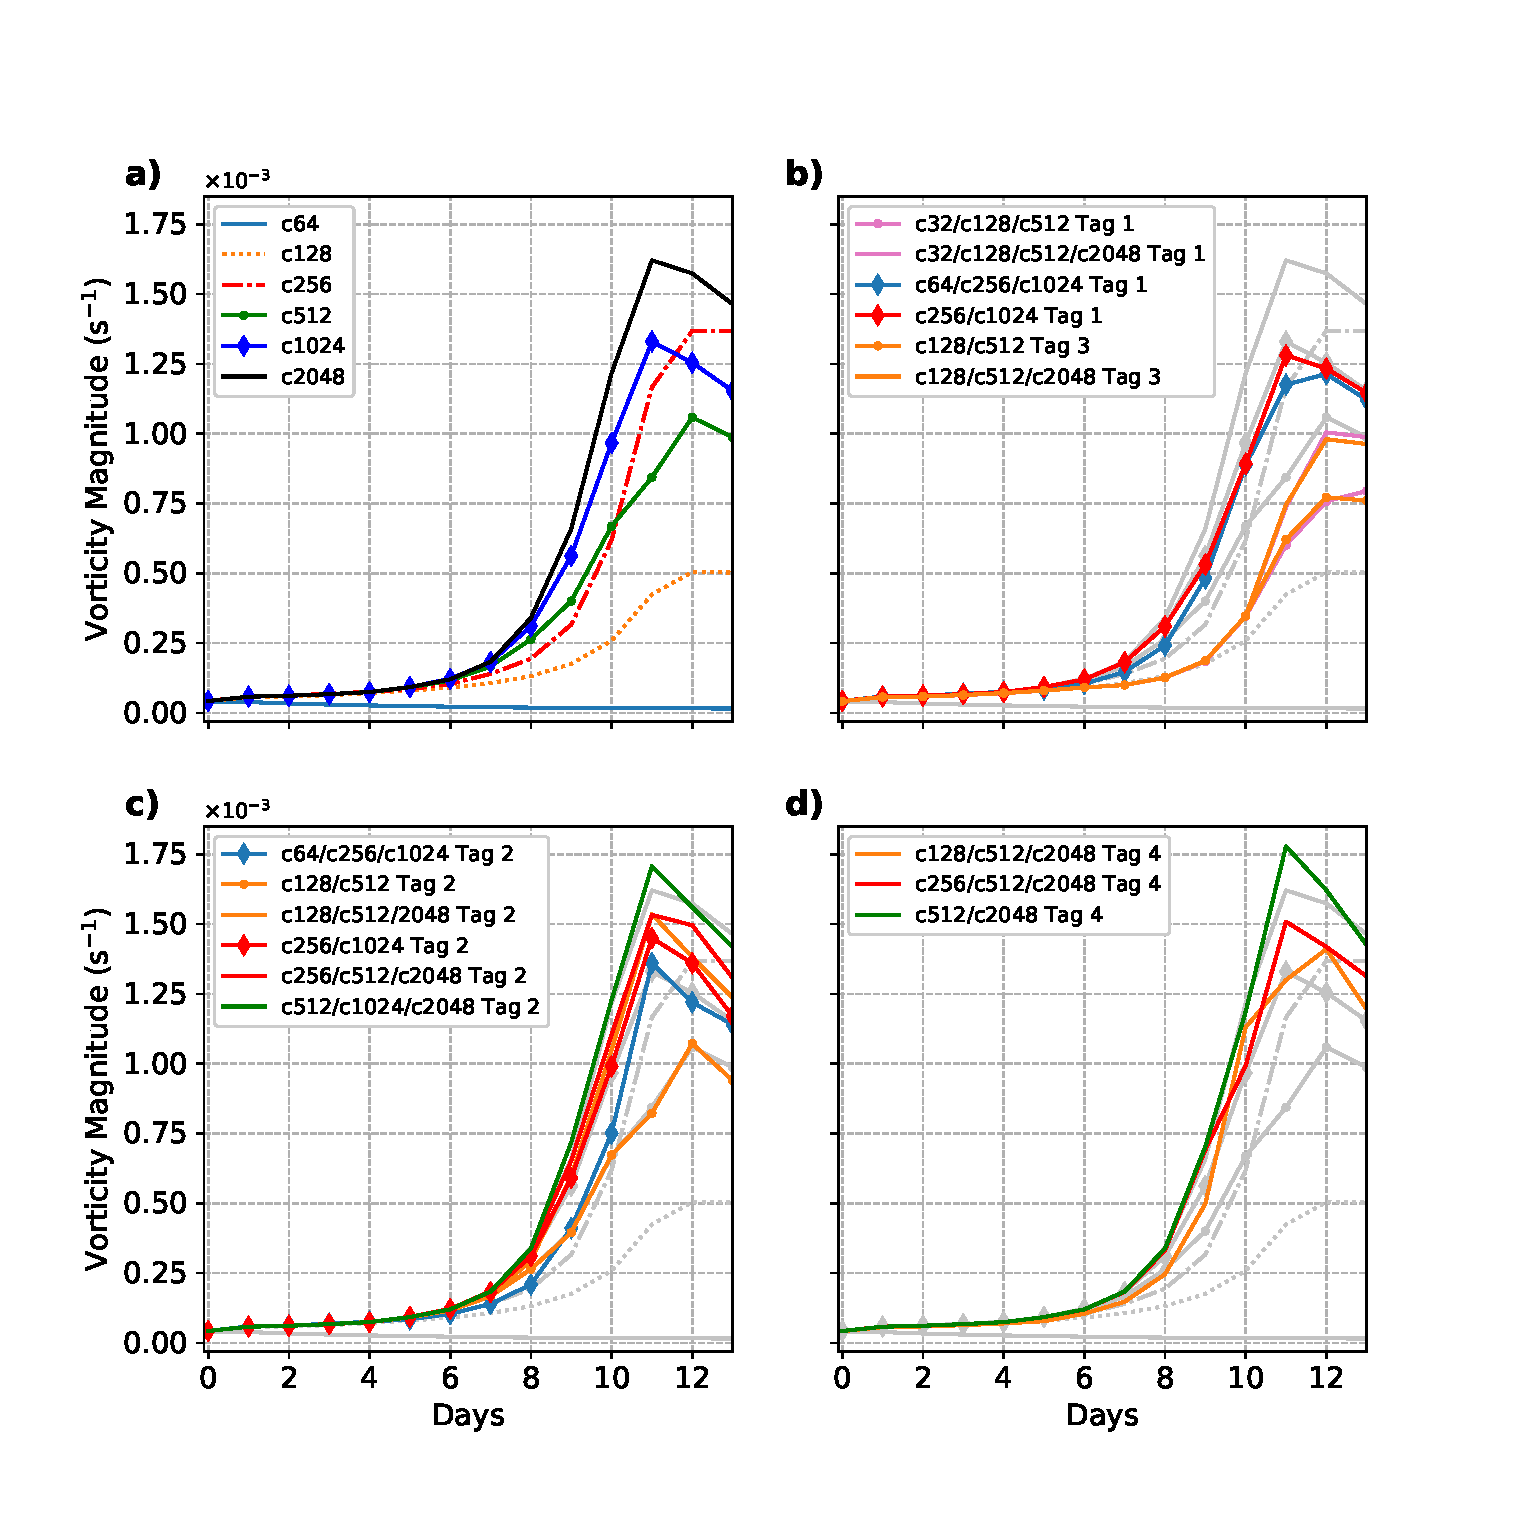
\includegraphics[width=\textwidth]{Chap2/vortmax_lineplot.eps}}
   \caption{Maximum relative vorticity of the strengthening vortex over a 
   period of 13 days for (a) uniform runs, (b) AMR runs using the Tag 1 or
   Tag 3 refinement criteria, (c) AMR runs using the Tag 2 criteria, and (d)
   AMR runs using the Tag 4 criteria. All the plots follow a line color and marker
   system dependent on resolution. The line color denotes the run's base resolution
   while the line style denotes the run's highest AMR resolution. The line color and
   style for each resolution is as follows: c2048 (black, plane), c1024 (blue, solid diamond markers),
   c512 (green, small circle markers), c256 (red, dot-dash line), and c128 (orange, dotted line).
   The coarse resolutions c64 and c32 have only a line color, light blue and pink respectively, and
   no line style as none of the AMR runs have a highest refinement at these resolutions given that
   the vortex does not develop on such a coarse grid (as seen by the c64 uniform run in (a)).
   For comparison purposes the uniform run lines from (a) have been imposed in light grey on
   the other three plots.
   }
   \label{fig:vort_lineplot}
\end{figure}

Overall stronger vortex with higher resolution with the higher resolution having larger
maximum vorticity for first nine day. The c64 resolution has not strengthening and 
neither did c32 resolution which is not plotted in Fig. \ref{fig:vort_lineplot}a. 
In these cases the grid resolution is
too coarse and the initialized vortices slowly weaken.
In Fig. \ref{fig:vort_lineplot} after day 9 we see the c256 run strengthening 
more rapidly than higher resolution runs so
that it has higher maximum vorticity than c512 run and c1024 run by day 12.  Over the same time 
period we see that the c512 and higher resolution runs reach a peak strength between day 11 and day 12
before slowly decreasing. Observing a regime change that coarser resolutions c256 and c128 are not
able to resolve. This regime change can be seen in Fig. \ref{fig:uni_d9nd12} which 
depicts the relative vorticity field for uniform runs c256, c512, and c1024 at day 9 
Figs. \ref{fig:uni_d9nd12} (a)-(c) and day 12 Figs. \ref{fig:uni_d9nd12}(d)-(f).

\begin{figure}
   \centerline{%
   \noindent
   \includegraphics[width=\textwidth]{Chap2/uni_runs_day9n12-01}}
   \caption{Relative vorticity field of the 
   strengthening vortex case at day 9 (a) - (c) and day 12 (d)-(f) for uniform runs 
   c256 resolution (a) and (d), c512 resolution (b) and (e), and 
   c1024 resolution (c) and (f) These plot
   correspond to the day 9 uniform c2048 plot, Fig. \ref{fig:c2048_vortseries}g, a
   day 12 plot Fig. \ref{fig:c2048_vortseries}i.
   }
   \label{fig:uni_d9nd12}
\end{figure}

Comparing day 9 in Fig. \ref{fig:uni_d9nd12} and Fig. \ref{fig:c2048_vortseries}g,
the strength of the vortex is clearly depend on resolution as the maximum vorticity
increases with each resolution. The structure of the vortex, however, visually 
converges. The ring collapse and roll-up seen at day 9 in the 
uniform c2048 run in Fig. \ref{fig:c2048_vortseries}g
is also observed in the c1024 run (Fig. \ref{fig:uni_d9nd12}c) 
despite the slightly weaker maximum vorticity.
The weaker vortex of the uniform c512 run results in a delay of the 
stretching and collapse of vortex ring. In Fig. \ref{fig:uni_d9nd12}b,
the vortex is stretched but the roll-up has not begun. The ring
structure is still visible but not as distinct as in the higher resolution runs.
In uniform c256 run the vortex does not form a distinct vortex ring structure 
and merely continues to strengthen at day 9 with out a significant
change to its structure. (Fig. \ref{fig:uni_d9nd12}a).

By day 12, in the c1024 the vorticity filaments have rolled back up into a single vortex and spun off
a smaller secondary vortex with a vorticity dipole feature. The field is visually
similar to c2048 run at day 12 in Fig. \ref{fig:c2048_vortseries}i, 
albeit slightly weaker over all and thus less further north by day 12. 
Since the the c256 run did not undergo the collapse and rollup,
its max vorticity at day 12 in Fig. \ref{fig:uni_d9nd12}d is now stronger 
than c512 and c1024 vortices.  In addition, no secondary vortex gets 
spun off.  The uniform c128 run follows a similar evolution, just weaker, so it is not shown here. 
For the c512 uniform run at day 12 in Fig. \ref{fig:uni_d9nd12}e, a secondary vortex has spun off 
(centered around $(25^\circ N, -3^\circ W)$ but its significantly weaker than the secondary vortices 
in the c1024 and c2048 runs. In addition, one of the two anticyclonic regions that abut the main 
vortex in the other high resolution runs has been spun off as well. Figure \ref{fig:uni_d9nd12}
shows these two difference regimes dependent on resolution. At resolutions c256 and below
the development of a distinct vortex ring and its collapse cannot be resolved. The c512
resolution appears to be the start of the high resolution regime, 
which starts to converge between the c1024 and c2048 resolution runs.

Returning to Fig. \ref{fig:vort_lineplot} and the AMR runs plotted in (b)-(d), the AMR runs do an 
effective job of following the growth trajectory of uniform run with the same resolution as 
the AMR run's finest level with a few exceptions.  As expected in several cases
the AMR run's maximum vorticity remains lower than the corresponding uniform run.
This occurs from higher resolution refinement not being implemented early enough
resulting in the lower strength evolution seen in the uniform c256 and below runs.
This can be seen in the c128/c512/c2048 AMR with Tag 4 in Fig. \ref{fig:vort_lineplot}d.
The refinement levels in that run are triggers starting at day 2, that resulting delay
results in the maximum strength remaining below the uniform c2048 level throughout
the thirteen days of simulation. The largest divergence occurs for the c32 AMR runs
with Tag 1 and c128 AMR runs with Tag 3 in Fig. \ref{fig:vort_lineplot}b. 
The two runs with a highest AMR level of c2048 have a maximum vorticity
nearly 40\% weaker at day 12 than the uniform c2048 run. The other two AMR runs with a highest
AMR level of c512 runs are approximately 25\% weaker than the c512 uniform vortex. These runs also 
follow the low resolution regime more closely than the their highest AMR level expected regime. 
All four of these runs begin with a highest resolution of c128, as the Tag 1 threshold for c32 AMR runs 
triggers the c128 level of refinement immediately at initialization.  However for both the c32 AMR tag 1 runs
and the c128 tag 3 runs, the c512 AMR level is not triggered until six and a half days into the simulation
and the c2048 level for the two runs that have it is not triggered until after day 10. As a result the 
improvements from having higher resolution occur too late. As Fig. \ref{fig:vort_lineplot}b shows, these four
runs don't diverge from the c128 uniform run until day 9. In other AMR setups, the delayed implementation of
the highest AMR resolution does not degrade the growth of the vortex strength. For the c64/c256/c1024 AMR 
runs with tag 1 and tag 2 refinement, the first refinement level of c256 resolution is triggered initial. However,
the second, c1024, level is not trigger until after five days for tag 1 and at seven days for tag 2.  As a result,
we observe that the c64 AMR run with tag 1 in Fig. \ref{fig:vort_lineplot}b does not diverge from the uniform c256
run until after day 7, and in Fig. \ref{fig:vort_lineplot}c the c64 tag 2 AMR run does not diverge until after day 8.
Both however follow the c1024 maximum vorticity closely by day 10.
Though delayed, the refinement still occurs before the rapid intensification period during which
the vortex ring that develops become unstable and collapses. Thus these runs are able to more successfully
match the c1024 uniform results than the c32 tag 1 AMR runs. In a few other cases, the AMR results in a 
slightly higher maximum vorticity than the corresponding uniform run. This occurs between day 10
and day 12 with the c512/c2048 AMR runs using 
Tag 2 (Fig. \ref{fig:vort_lineplot}c) and Tag 4 (Fig. \ref{fig:vort_lineplot}d)  
as well as with the c256/c1024 AMR run using Tag 2 (Fig. \ref{fig:vort_lineplot}c).

\begin{figure}
   \centerline{%
   \noindent
   \includegraphics[width=\textwidth]{Chap2/day9_vort-01.eps}}
   \caption{Relative vorticity fields at day 9 for several AMR runs of the 
   strengthening vortex case. (a) c32 base 4-level AMR run with x4 
   refinement using Tag 1. (b) c128 base 3-level AMR run with
   x4 refinement using Tag 3.
   (c) c256 base 2-level AMR run with x4 refinement using Tag 2.
   (d) c64 base 3-level AMR run with x4 refinement using Tag 1.
   (e) c128 base 3-level AMR run with x4 refinement using Tag 2.
   (f) c256 base 3-level AMR run with one level of x2 refinement 
   and one of x4 refinement using Tag 2.
   (g) c64 base 3-level AMR run with x4 refinement using Tag 2.
   (h) c128 base 3-level AMR run with x4 refinement using Tag 4.
   (i) a c512 base 2-level AMR run with x4 refinement using Tag 4. These plots
   correspond to the day 9 uniform plots in Fig. \ref{fig:c2048_vortseries}g and
   \ref{fig:uni_d9nd12}(a)-(c). The block structures of the multiple refinement
   levels are outlined in black
   }
   \label{fig:vort_amr_day9}
\end{figure}

Figures \ref{fig:vort_amr_day9} and \ref{fig:vort_amr_day12} depict the relative 
vorticity field for day 9 and day 12 respectively for nine AMR runs. They provide 
for a more detailed comparison of overall vortex and small scale features in the 
vorticity field between the AMR runs and the uniform resolution runs in 
Fig. \ref{fig:c2048_vortseries} and Fig. \ref{fig:uni_d9nd12}. At day 9, the selected
AMR runs in Fig. \ref{fig:vort_amr_day9} are at various stages of the 
evolution process depending on their resolutions and tagging criteria. As in 
Fig. \ref{fig:vort_lineplot}b, the c32 base 4-level AMR with Tag 1 run (Fig. 
\ref{fig:vort_amr_day9}a) and the c128 3-level AMR with Tag 3 run (Fig.
\ref{fig:vort_amr_day9}b) are significantly weaker than the uniform c2048 run
at day 9 (Fig. \ref{fig:c2048_vortseries}g). The highest level of AMR for both runs, c2048,
has not been triggered yet and both runs have on c512 resolution over the vortex.
 The evolution of the vortex is following the high resolution regime, with the clearly visible
 vortex ring, it is just delayed. Figures \ref{fig:vort_amr_day9}a and b are more comparable to
the c2048 uniform run at day 6 (Fig. \ref{fig:c2048_vortseries}d). Though not as pronounced,
the two c64 based AMR runs are also delayed in their vortex evolution. The c64 3-level AMR runs
with tag 1 (\ref{fig:vort_amr_day9}d) and tag 2  (\ref{fig:vort_amr_day9}d) both have a clearly
defined vortex ring that has begun to stretch and deform. However, they are more similar 
in strength and appearance to the c512 uniform run at day 9 in Fig. \ref{fig:uni_d9and12}b. 
In addtiion, the vortex in the c64 tag 1 run is slightly stronger and more deformed reflecting the
two day advantage in when the c1024 AMR level is triggered that the lower threshold
gives the tag 1 run.

The c128 and higher resolution base level AMR runs are able to capture the vortex roll-up
effectively at day 9. The three AMR runs using the tag 2 refinement criteria, 
the c256/c1024 run (Fig. \ref{fig:vort_amr_day9}c), the c128 3-level 2 AMR run
(Fig. \ref{fig:vort_amr_day9}e), and the c256 3-level AMR run (Fig. \ref{fig:vort_amr_day9}f),
as well as the c512 2-level AMR tag 4 refinement criteria run (Fig. \ref{fig:vort_amr_day9}i)
capture the collapse and roll up of the vortex and closely match the vorticity magnitudes
 in the c1024 and c2048 uniform runs at day 9. 
The AMR runs are also able to resolve  the two areas of negative vorticity 
on either side of the main vortex. However, the roll up process in the AMR is slightly
behind that of the high resolution uniform runs. The distinct comma like positive vorticity 
feature of the main vortex ring seen in the uniform c2048 (Fig. \ref{}g) and c1024 (Fig. \ref{}c) runs
is not as prominent yet in these AMR runs. 
The exception is the c128 base 3-level AMR run with tag 4. Seen in
Fig. \ref{fig:vort_amr_day9}h, the vortex ring in this tag 4 run 
is about 25\% weaker as noted in Fig. \ref{fig:vort_lineplot}d than the c2048 uniform run and  the vortex
roll up is about half a day behind. The slightly deformation in the ring and the positive vorticity filament 
extending northward from the northwest sector of the vortex ring, corresponds well to structure of
the vortices in the uniform c1024 and c2048 runs at 8.5 days. 

\begin{figure}
   \centerline{%
   \noindent
   \includegraphics[width=\textwidth]{Chap2/day12_vort-01.eps}}
   \caption{Same as Fig. \ref{fig:vort_amr_day9}, but for day 12 after the small
   secondary vortex has spun off. These plots correspond to the day 12 uniform
   plots in Fig. \ref{fig:c2048_vortseries}i and \ref{fig:uni_d9nd12}(d)-(f). Once
   again the block structures of the multiple refinement
   levels are outlined in black
   }
   \label{fig:vort_amr_day12}
\end{figure}

Figure \ref{fig:vort_amr_day12} depicts the vorticity fields for the AMR runs after the vortex ring collapse
and spin off of a smaller secondary vortex. The c256 and c512 base resolution AMR runs (Figs.
\ref{fig:vort_amr_day12}c, f, and i) have vorticity 
maximums roughly 10\% higher than their corresponding high resolution 
uniform runs reflecting Fig. \ref{fig:vort_lineplot}. These three AMR runs are also match
the formation and location of the secondary vortex most closely and capture the anticyclonic
 filaments wrapping aground the main vortex.
The other six coarser base resolution AMR runs have lower peak magnitudes. The 
vorticity fields for the c32 tag 1 AMR run in Fig. \ref{fig:vort_amr_day12}a and the
c128 tag 3 AMR run in Fig. \ref{fig:vort_amr_day12} show a delayed spin off of 
a secondary vortex and less symmetric main vortex more 
comparable to day 10 of the c2048 uniform run in Fig. \ref{fig:c2048_vortseries}h.
The c64 3-level AMR tag 1 run in Fig. \ref{fig:vort_amr_day12}d has a vorticity 
maximum similar to the c1024 uniform reference. The AMR run also resolves 
the secondary vortex, though its position is further to the northwest than shown
in Fig. \ref{fig:uni_d9nd12} for day 12 in the c1024 uniform run. In contrast,
the slightly higher threshold in the tag 2 refinement criteria 
for the c64 3-level AMR run (Fig. \ref{fig:vort_amr_day12}g) 
is unable to reproduce the secondary vortex spinning off. The
c128 AMR runs depicted in Fig. \ref{fig:vort_amr_day12}e and h both
a secondary vortex developing, though the tag 2 run's is more chaotic.
The area around the tag 2 run's secondary vortex has large negative 
vorticity filament and a weak third cyclonic vortex.
The anticyclonic filaments are also more define in Fig. \ref{fig:vort_amr_day12}h 
than in e. 

\begin{figure}
   \centerline{%
   \noindent
   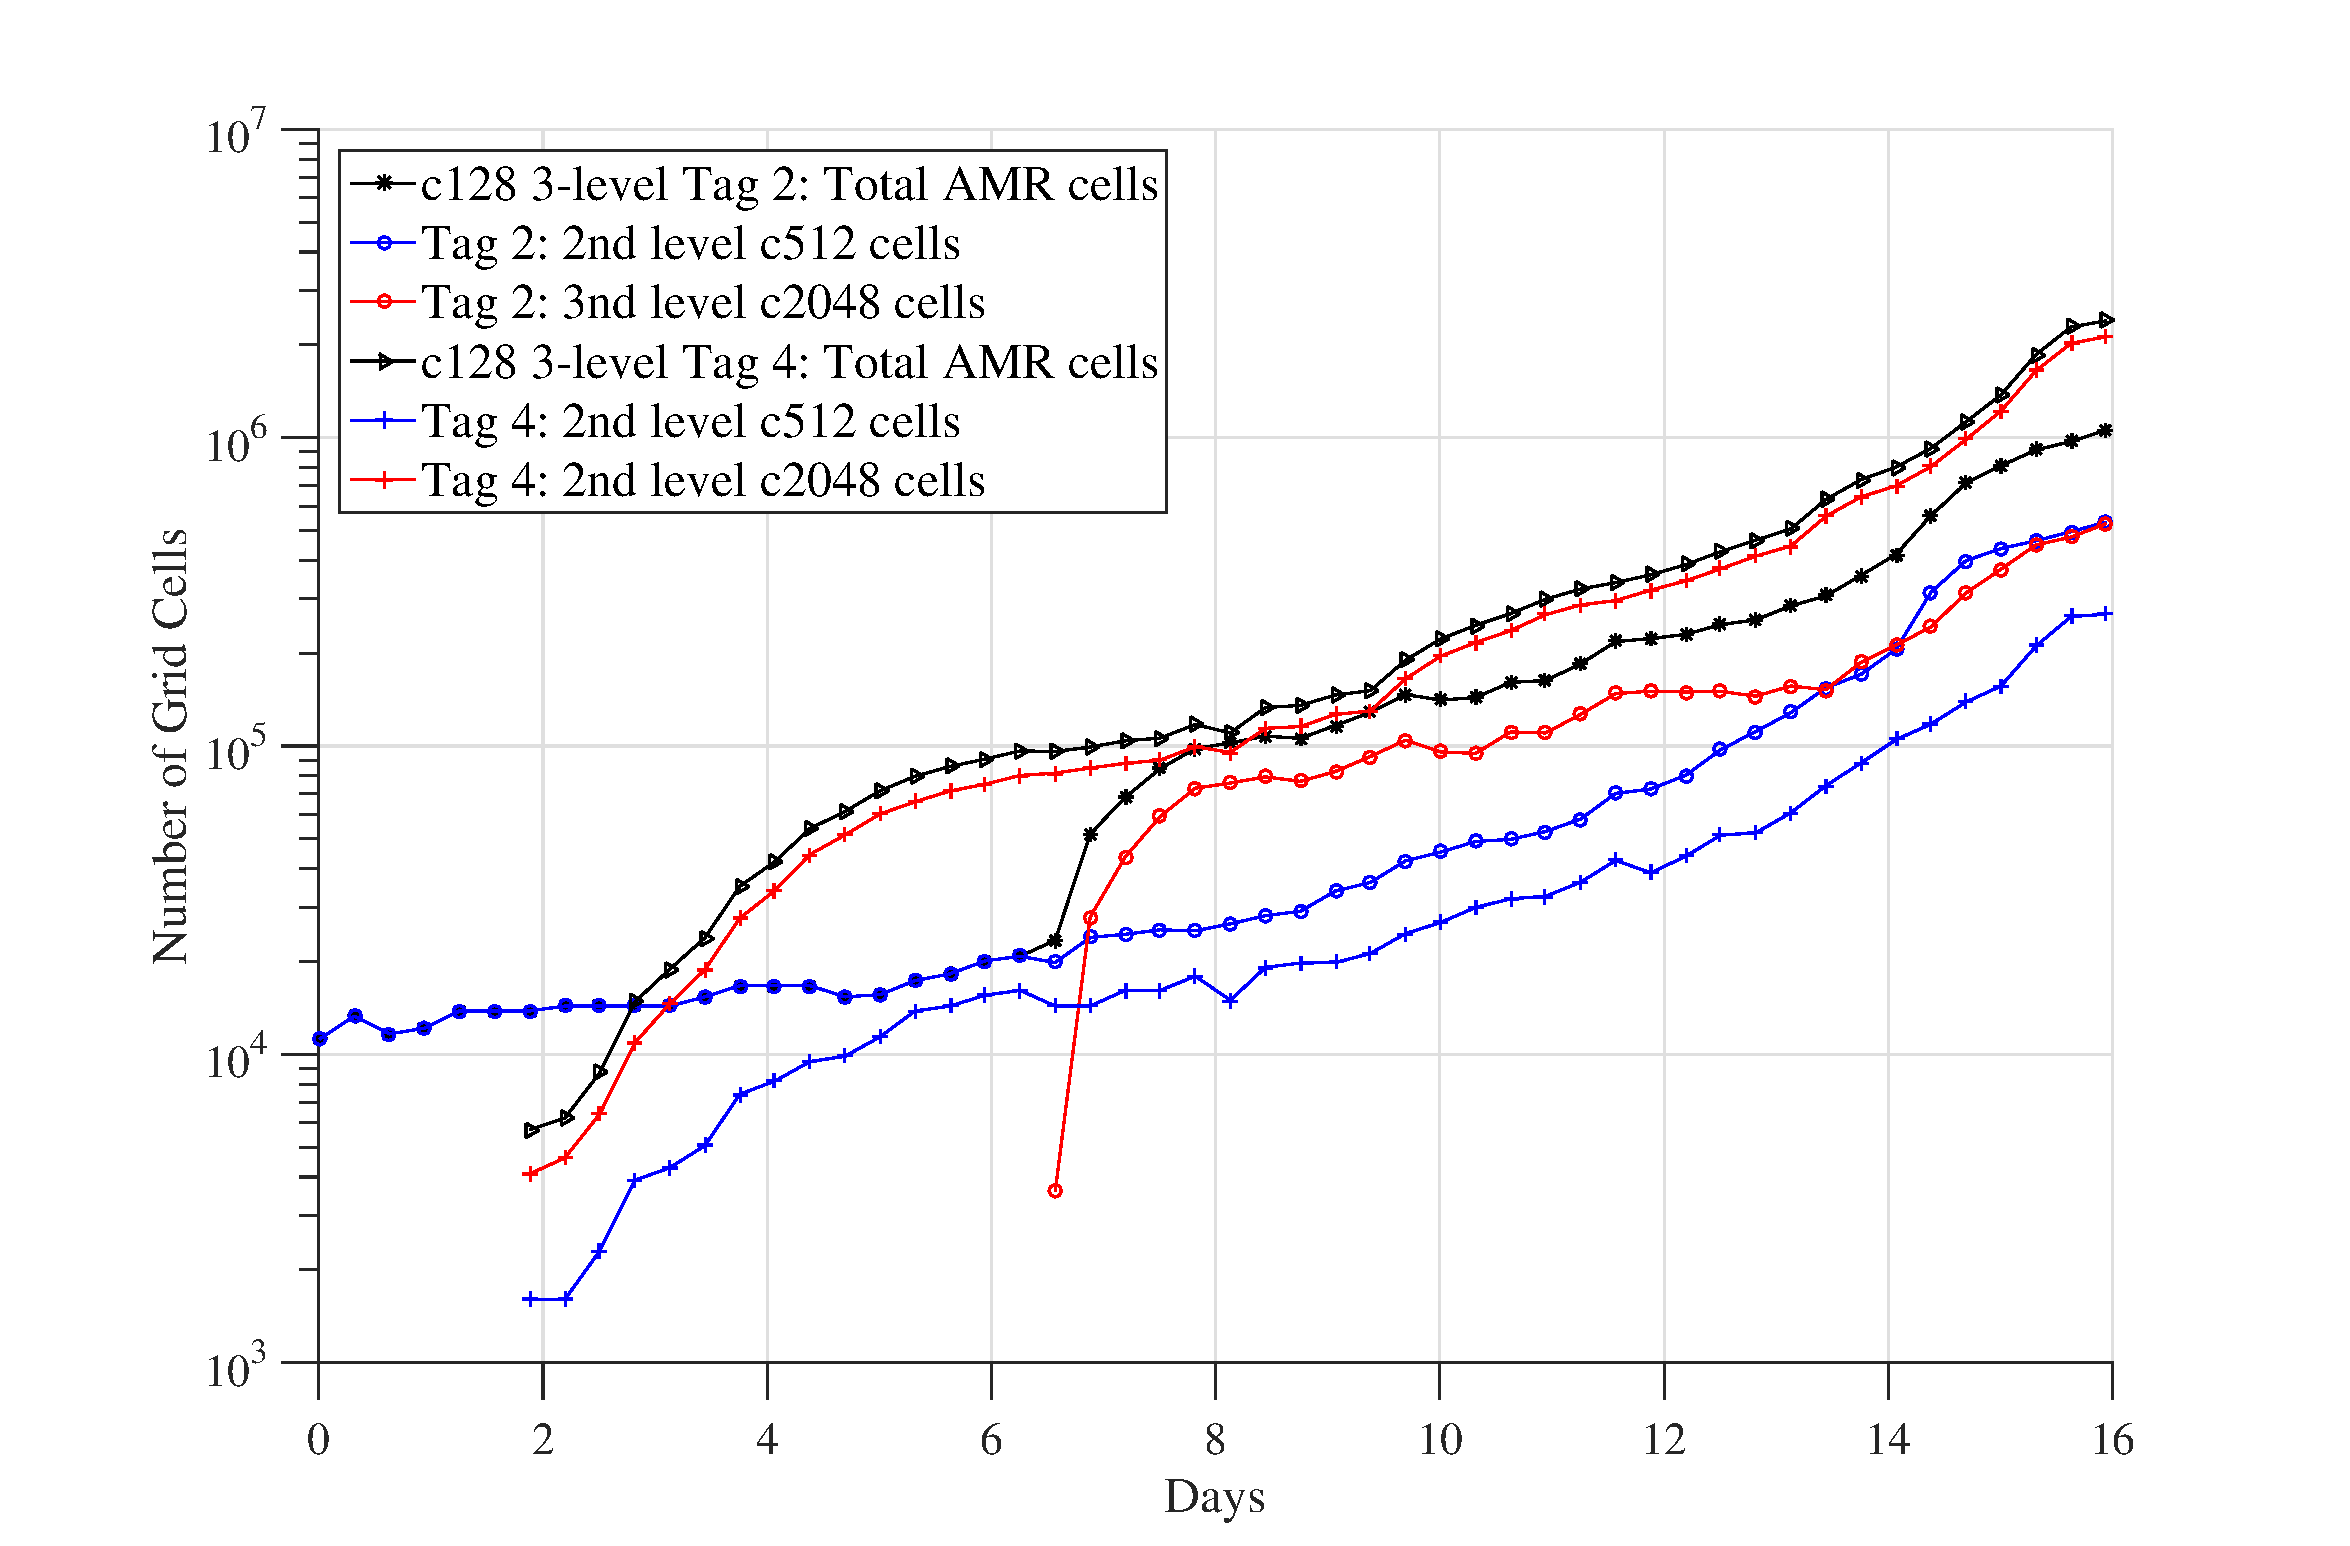
\includegraphics[width=\textwidth]{Chap2/c128_3l4_Tag2vs4_compare.eps}}
   \caption{The growth of AMR grid cells over time for the two c128 3-level AMR runs 
   with tag 2 and tag 4 refinement criteria. The base level c128 grid cells are exclude
   while the 2nd level c512 cells are plotted in blue and the third level c2048 cells are
   plotted in red with a plus marker to denote the tag 4 run and a circle to denote the
   tag 2 run.  The sum of the two levels are plotted in black with a triangle marker denoting
   the tag 4 run and an asterik marking the tag 2 run. 
   }
   \label{fig.grid_num_c128}
\end{figure}

Figure \ref{fig.grid_num_c128} shows the number of grid cells at each AMR 
level as a function of time for both c128 3-level AMR runs.  While, the lower 
base level refinement threshold in tag 2 results in c512 level AMR being applied
initially. It takes two days for refinement to occur with the tag 4 criteria at which time
due to the constant threshold value both levels of refinement are implemented.
Though the c2048 refinement level 
covers only the center core of the vortex. The outer edges of the vortex remain at
c512 or even c128 resolution for another day.
After day 3, the tag 4 run has nearly an order of magnitude more cells until the c2048
level is triggered for the tag 2 run after day 6. Once triggered,  the gap narrows significantly. 
Through the entire 16 day simulation the tag 2 run has more level 2 c512 grid
cells while the tag 4 run has more c2048 cells. So though the c128 3-level AMR tag 4 run
has more grid cells and the c2048 refinement level for four more days than the 
c128 3-level AMR tag 2 run, the tag 2 run does a better job of capturing the vortex roll up at day 9 
(Figs. \ref{fig:vort_amr_day9}e and h).
That extra c512 resolution for the first two days appears to outweigh the benefits 
of having the more c2048 resolution throughout the majority of the run time. 
The benefit of that early advantage fades as the run continues, and the benefit of more coverage by
the c2048 refinement level becomes apparent. By day 12 
the c128 tag 2 run is lacking the c2048 resolution around the core of the main 
vortex needed to resolve the thin negative vorticity filaments (Fig. \ref{fig:vort_amr_day12}e), 
which the tag 4 run is able to capture (Fig. \ref{fig:vort_amr_day12}h). 
The secondary vortex in the tag 4 run also more close resembles the uniform c2048 run.

A key delineator between these AMR runs is when refinement with c512 resolution or
higher is implemented. With c512 or greater resolution, the vortex undergoes the evolution regime for
the high uniform resolutions.  The AMR runs that criteria that triggered refinement levels 
of at least c512 initially or within the first day had vortex growth most similar to the uniform c2048. 
Even when these runs did not trigger additional higher levels refinement like c2048
until day six or later, they still performed better than AMR runs that trigger c2048 refinement
much earlier but not a resolution below c512 over the vortex for the first few days.  
Resolution added later in the simulation still improved the results, and we do observe 
rapid strengthening and switching of evolution regimes once
 refinement c512 or higher is triggered. The critical vortex collapse merely occurs later in time and we
see some of those AMR runs do have adequate time to "catch-up" to the reference solution run by day 10 
or 12.

     \subsection{Extended Run Results}
Extending the simulation time leads to an active and complex global flow pattern developing.
The isolated vortex discussed in detail in the previous sections and the binary
pair of weaker vortices also initialized evolve independently of each other for twelve days. 
Beyond twelve days, the Rossby wave trains though small in magnitude
spread triggering evaporation and convection over a significant area.
As a result by day 16 of the simulation a global chaotic flow has developed with multiple
cyclonic and anticyclonic areas developing unseeded.  Additionally, jet like features
develop around the $30^\circ$N and S latitudes corresponding to the areas 
where the initial moisture field and moisture reservoir transition from high levels
near the equator and low levels near the poles. 
Figure \ref{fig:threevort_uni} depicts a snapshot vorticity field of all three vortices 
at day 9 and day 12 and the resulting global vorticity field at day 16
for uniform c256 (Fig. \ref{fig:threevort_uni}a), c512 (Fig. \ref{fig:threevort_uni}b),
c1024 (Fig. \ref{fig:threevort_uni}c), and c2048 (Fig. \ref{fig:threevort_uni}d) resolution
runs. The plots for day 9 and 12 are zoomed in to focus on the three vortices since
these are the primary features during that time frame. Day 16 plots depict the 
global relative vorticity field. The over all flow, the number of large-scale vortices
and their location remain fairly consistent across the increasing uniform resolutions.
The higher resolutions naturally resolve more fine-scale structures in this chaotic system.
The uniform c1024 and c2048 also resolve several small-scale vortices (Observe the small 
cyclonic vortex around $15^\circ$N and $30^\circ$W in the c1024 and c2048 run and 
the several anticyclonic patches nearby). The sharp increase in maximum vorticity
in the c2048 run at day 16 is from the cyclonic vortex pointed out.

\begin{figure}
   \centerline{%
   \noindent
   \includegraphics[width=\textwidth]{Chap2/global_uni_vort-01.eps}}
   \caption{Late run evolution of the relative vorticity field for the 
   strengthening vortex case with three initialized vortices. These plots show
   the growth of a global chaotic regime by day 16 in for uniform resolution
   runs. Relative vorticity snapshots at days 9 (left column), 12 (middle column), 
   and 16 (right column) are given for
   (a) uniform c256 run, (b) uniform c512 run, (c) uniform c1024 run, and
   (d) uniform c2048 run. The left most vortex in the days 9 and 12 plots
   located around $(30^\circ \mathrm{N}, 15^\circ \mathrm{W})$ is the isolated
   vortex discussed in previous sections. The two vortices centered around
   $(20^\circ \mathrm{N}, 90^\circ \mathrm{E})$ are the binary pair. Note: the
   vorticity extrema occur in the isolated vortex in all cases for days 9 and 12 so they are 
   not displayed.}
   \label{fig:threevort_uni}
\end{figure}
\begin{figure}
   \centerline{%
   \noindent
   \includegraphics[width=\textwidth]{Chap2/day16_vort-01.eps}}
   \caption{Relative vorticity fields at day 16 for four AMR runs of the strengthening
   vortex case with three initialized vortices: 
   (a) c64 base 3-level AMR run with x4 refinement using Tag 2,
   (b) c128 base 3-level AMR run with x4 refinement using Tag 2,
   (c) c256 base 2-level AMR run with x4 refinement using Tag 2,
   and (d) c256 base 3-level AMR run with one level of x2 refinement 
   and one of x4 refinement using Tag 2. The left column depicts the vorticity 
   field at day 16 while the right column overlays
   the block structures of the refinement levels in black. These plots
   are comparable to the day 16 plots in Fig. \ref{fig:threevort_uni}.
   }
   \label{fig:vort_amr_day16}
\end{figure}

In addition to the uniform runs, we extend four AMR runs out to 16 days. 
The global vorticity fields at day 16 for the four AMR runs are plotted in 
Fig. \ref{fig:vort_amr_day16}. The first column depicts the relative vorticity,
while the second column shows the block structure for the multiple AMR levels.
All four AMR runs do an effective job of capturing the overall flow of the system.
The c64 base 3-level AMR run in Fig. \ref{fig:vort_amr_day16}a captures all the features
with its intermediate AMR level. However, the highest c1024 level is limit to the main vortices
and a few of the larger filaments. Thus much of the secondary flow and small scale features 
features in this chaotic system diverge from the high resolution uniform runs. The c128 base
3-level AMR run in Fig. \ref{fig:vort_amr_day16}b, the c256/c1024 AMR run in Fig. 
\ref{fig:vort_amr_day16}c, and the 3-level c256/c512/c2048 AMR run in Fig.
\ref{fig:vort_amr_day16}d all have a high resolution level over much of the area that
is better able to capture the small scale filaments and features. The one key area of
where the latter three AMR runs differ from their corresponding highest resolution
uniform run is in the maximum vorticity. In the AMR runs like the c1024 and c2048 
uniform runs the vorticity maximums and minimums are from the small scale vortices
that develop. However these extrema values for the AMR runs in Figs. 
\ref{fig:vort_amr_day16}b, c, and d are more than double the uniform runs' values.
The $2.53 \times 10^{-3}\mathrm{s}^{-1}$ maximum in the c128 three-level run and
the $3.81 \times 10^{-3}\mathrm{s}^{-1}$ maximum in the c256 three-level run are
from small scale vortices with small patches of the highest level of refinement.  However
the equally large compared to it's uniform run comparison 
$1.8 \times 10^{-3}\mathrm{s}^{-1}$ maximum in the c256/c1024 AMR run is centered
in a broad area of refinement that had been under refinement for several days. These vortices
are well resolved with more the ten grid cells across and a significant buffer of refinement between the
vortices and the coarse-fine boundaries. So it
seems unlikely that these large vorticity values are being formed AMR level boundaries.
The cause is more likely to be the chaotic nature of this system sixteen days out. The flow
flow difference between the runs are likely enough to trigger these small vortices.

%%%%%%%%%%%%%%%%%%%%%%%%%%%%%%%%%%%%%%%%%%%%%
\section{Kessler-like Physics for Shallow Water Equations}
An alternative setup for a moist forced shallow water system presented in 
\cite{zerroukat2015moist} derives the 2D shallow water equations from 
the moist Boussinesq equations. It includes a three-state moist physics 
model that simulates water vapor, cloud vapor, and liquid water, 
similar to the simplified 3D physics scheme prseneted in 
\cite{kessler1969distribution}. The forcing setup
is comparable to the generalized shallow water equations or Ripa's 
model \citep{ripa1993conservation,ripa1995improving} 
used in ocean modeling and other fields.  
In this model, latent heat released due to precipitation increases 
the average potential temperature of the fluid, which is coupled
to momentum equations.  The model can be viewed as a
diabatic non-convective model in contrast to the previous
model setup which can be considered an adiabatic convective 
model. It assumes energy released during
perception has no effect on the temperature and instead 
produces convection represented as a mass flux. A
brief discussion comparing the two models
is presented in Appendix A of \cite{bouchut2009fronts}.
We implement this physics forcing for both uniform and
AMR runs of the barotropic instability test case of
\cite{galewsky2004initial}.

\subsection{The Shallow Water and Physics Equations}
\cite{zerroukat2015moist} dimensionally reduces the Boussinesq equations 
to obtain a derivation of the shallow water equations that retain some
buoyancy terms. These shallow water equations are presented below in flux-form:
   \begin{equation}
     \label{eq:swkesmom} \frac{\partial h \mathbf{v}}{\partial t} +
     \nabla \cdot (h \mathbf{v} \mathbf{v}) + f \mathbf{\hat{k}}\times(h\mathbf{v}) + gh\nabla H = 
     g h \theta \nabla h_b + g\nabla (\frac{1}{2}h^2\theta)
   \end{equation}
   \begin{equation}
     \label{eq:swkescon}  \frac{\partial h}{\partial t} + \nabla \cdot (h\mathbf{v}) = 0
   \end{equation}
   \begin{equation}
     \label{eq:swthetacon}  \frac{\partial h\theta}{\partial t} + \nabla \cdot (h \theta \mathbf{v}) = hS_\theta
   \end{equation}
   \begin{equation}
     \label{eq:swkesqcon}  \frac{\partial h q^{(k)}}{\partial t} + \nabla \cdot (h  q^{(k)} \mathbf{v}) = hS_q^{(k)}
   \end{equation}
where $H$ is total height, $h_b$ is the bottom topography height, $\theta$ is the temperature based 
quantity, $q^{(k)}$ represent the moist physics tracers, and $S_\theta$ and $S_q^{(k)}$ are 
the depth averaged moisture and temperature sources respectively. 
    
   The \cite{zerroukat2015moist} physics scheme consists of three forms of water vapor, 
$q_v$, cloud $q_c$, and rain $q_r$.  Whenever the local value of $q_v$ exceeds a 
prescribed function for saturation $q_{sat}(h, \theta)$, a fraction of the 
oversaturation is condensed into cloud, $\Delta q_v$ with a corresponding latent 
heat release that increases the temperature $\theta$ locally. In the same manner, 
if cloud is present in unsaturated air a fraction of the cloud evaporates, $\Delta q_c$ 
with a corresponding cooling effect. In both cases, only a fraction of the water is 
converted to avoid a two time step oscillation between oversaturated and sub-saturated 
air, caused by the changing temperature. Cloud can also be converted to rain when $q_c$ 
passes a prescribed threshold $q_{precip}$ and a fraction of the excess cloud is then 
converted to rain, $\Delta q_r$. In this setup, only $q_v$ and $q_c$ are advected as 
tracers as $q_{(k)}$ in Eq. \ref{eq:swkesqcon}. Once cloud mositure is transformed 
into rain it is removed from the system. Processes such as rain evaporation and 
accretion are neglected in this simplified model are neglected. The equations for 
these processes and the source terms for the moisture variables 
($S_q^{(1)}=S_{q_v}, \,\, S_q^{(2)}=S_{q_c}$) from Eq. \ref{eq:swkesqcon} 
and temperature $S_\theta$ from Eq. \ref{eq:swthetacon}.
   \begin{eqnarray}
     \Delta q_v & = & \frac{1}{\Delta t}\max \left[ 0, \gamma_v\left(q_v - q_{sat}\right)\right]\\
     \Delta q_c & = & \frac{1}{\Delta t}\min\left[ q_c, \max \left[0, \gamma_v\left(q_{sat} - q_v \right)\right]\right] \\
     \Delta q_r & = & \frac{1}{\Delta t}\max \left[ 0, \gamma_r\left(q_c - q_{precip}\right)\right]\\
     S_{q_v} & = & \Delta q_c - \Delta q_v \\
     S_{q_c} & = & \Delta q_v - \Delta q_c - \Delta q_r \\
     S_{\theta} & = & L\left(\Delta q_v - \Delta q_c\right)\,.
   \end{eqnarray}
The constant $\gamma_r$ is the rain conversion rate and $L$ is a pseudo-latent heat 
constant for the $\theta$ variable. As derived in \cite{zerroukat2015moist} the 
$q_{sat}(h, \theta)$, the saturation threshold, and $\gamma_v$, the $\theta$-dependent 
conversion rate between vapor and cloud moisture are:
   \begin{equation}
     \label{eq:qsat} q_{sat} = \frac{q_0}{gH}\exp{20\theta}
   \end{equation}
   where $q_0$ is a test case dependent constant set to have the initial max $q_v=0.02$ and
   \begin{equation}
     \label{eq:gammav} \gamma_v = \left(1 + L \frac{\partial q_{sat}}{\partial \theta}\right)^{-1} \, .
   \end{equation}
Given the simplicity of the model, the constants can be arbitrarily chosen. 
However, we use the realistic values chosen in \cite{zerroukat2015moist}, 
where $L=10$, $\gamma_r = 10^{-3} \mathrm{ s}^{-1}$, and $q_{precip} = 10^{-4}$. 
The model does not have a sink for $q_r$, and instead $q_r$ can be viewed 
as water being suspend in the air and advected around. Additionally, there
is no evaporation of $q_r$ in this setup, though the equations can be 
easily modified to make the phase-change model more complex. It is also
important to note that for these simulation the Chombo-AMR model does
not preserve monotonicity and no filters are applied. So, 
negative under shoots can occur in the tracer fields.
  
\subsection{Barotropic Instability Test Case Initialization}
The barotropic instability test case of \cite{galewsky2004initial} 
consists of a balanced zonal jet centered at $45^\circ$ N to 
which a small height perturbation is added to initiate the role up
of the jet. The initial velocity and height fields along with the height
perturbation are defined in \cite{galewsky2004initial}.
We add to that initialization the
$\theta$ and $q_v$ profiles, while $q_c$ and $q_r$ are set to zero everywhere.  
The initial $\theta$ profile is a quadratic function with a north-south variation
     taken from \cite{zerroukat2015moist} so that
   \begin{equation}
     \label{eq:pottemp}
     \theta(\phi, \lambda) = \theta^{SP}\left(\phi - \frac{\pi}{2}\right)\phi - 
     \left(1 - \mu_1 \theta^{EQ}\right)\left(\phi + \frac{\pi}{2}\right)\left(\phi - \frac{\pi}{2}\right)
     + \theta^{NP}\left(\phi + \frac{\pi}{2}\right)\phi.
   \end{equation}
The constants used for this test case are $\mu_1 = 2\times 10^{-5} $, 
$\theta^{SP}= -40\epsilon$, $\theta^{EQ}= 30\epsilon$,
and $\theta^{NP}= -20\epsilon$ where $\epsilon = 1 / 300$. The initial moisture profile 
is set just below the saturation level so $q_v(\phi, \lambda) = 0.98 q_{sat}(h, \theta)$, 
where $q_{sat}(h, \theta)$ is established from Eq. \ref{eq:qsat}, where $q_0 = 0.0492238$. 

\subsection{Effects of resolution in the moist barotropic instability test case}
The growth of the instability in the jet and evolution of the initial vorticity
roll-ups into sharp gradients is consistent with the results in \cite{galewsky2004initial}.
Significant cloud formation $q_c$ does not begin until after four days and that $q_c$ 
does not precipitate until five days into the simulation. By day six, the barotropic
wave has created distinct vortices and thin vorticity filaments. Within these front and
cutoff low-like features, areas of cloud and rain have formed. Figure \ref{fig:c2048allvar}
shows several variable fields for the baortropic wave at day 6 for
a uniform c2048 ($~5$ km). The potential
temperature $\theta$ in Fig. \ref{fig:c2048allvar}a and water vapor $q_v$ in
Fig. \ref{fig:c2048allvar}b echo the structure of the vorticity field 
(shown in Figs. \ref{fig:c2048allvar}c and d as black solid and dashed contour lines).
The protrusions of colder and drier areas within the vorticity troughs mimic frontal
systems. The $q_c$ field is depicted in Fig. \ref{fig:c2048allvar}c, while
Fig. \ref{fig:c2048allvar}d shows the total amount of water precipitated, $q_r$, 
in the preceding twelve hours. The highest areas of cloud and rain are 
within these vorticity troughs with weaker concentrations of $q_c$ located around
the cutoff lows.

\begin{figure}
   \centerline{%
   \noindent
   \includegraphics[width=\textwidth,height=\textheight,keepaspectratio]{Chap2/A_c2048_allvar-01}}
   \caption{Day 6 snapshots of the evolving barotropic wave for the c2048 uniform 
   run's (a) temperature field, (b) $qv$ moisture field, (c) $qc$ cloud field, (d) past 12-hour 
   accumulation of the $qr$ precipitated water field. The solid and dashed black contour
   lines in (c) and (d) represent the positive and negative relative vorticity respectively.
   The spacing between contour lines is $ \mathrm{s}^{-1}$.
   }
   \label{fig:c2048allvar}
\end{figure}

The effects of resolution and variable refinement on the barotropic instability's vorticity
field has been well covered (see \cite{st2007comparison}, \cite{Weller:2009gl}, 
and \cite{scott2016test}). So, we focus our investigation on how the physics
scheme's cloud $q_c$ and precipitation are affected by changing resolution
and AMR. The $q_c$ fields at day 6 for four other uniform resolutions: c128, c256, c512, and
c1024 are depicted in Fig. \ref{fig:uniformqc} for comparison with the c2048 run $q_c$ plot 
in Fig. \ref{fig:c2048allvar}c. The accumulation of precipitated water $q_r$ over
a half day period before day 6 for the four uniform resolutions is plotted in Fig. \ref{fig:uniformqrdt}
and corresponds to Fig. \ref{fig:c2048allvar}d for the uniform c2048 run.

\begin{figure}
   \centerline{%
   \noindent
   \includegraphics[width=\textwidth,height=\textheight,keepaspectratio]{Chap2/A_qc_uniform-01}}
   \caption{Plots of the $qc$ cloud field at day 6 for several 
   uniform resolutions: (a) c128, (b) c256, (c) c512, and (d) c1024.The c2048 uniform run
   plot of the same field in Fig. \ref{fig:c2048allvar}c serves as a reference.
   }
   \label{fig:uniformqc}
\end{figure}

\begin{figure}
   \centerline{%
   \noindent
   \includegraphics[width=\textwidth,height=\textheight,keepaspectratio]{Chap2/A_qrdt_uniform-01}}
   \caption{Plots depicting the 12-hour accumulation in the $qr$ precipitated water field for
   (a) c128, (b) c256, (c) c512, and (d) c1024 uniform runs. The c2048 uniform run
   plot of the same field in Fig. \ref{fig:c2048allvar}d serves as a reference.
      }
   \label{fig:uniformqrdt}
\end{figure}

Cloud cover area is fairly consistent across all resolutions in Fig. \ref{fig:uniformqc}
The structure of the cloud field and even the smaller scale features centered on the cutoff 
lows and the left most wave converge at resolutions of c512 and higher. A key
difference in cloud cover structure is in the c128 run in Fig. \ref{fig:uniformqc}a.
The c128 run has two extra areas of cloud cover between $80^\circ$ and
$170^\circ$ longitude. These are an artifact of the cubed-sphere grid.
As observed by \cite{st2007comparison} and \cite{ullrich:2010vn}, the barotropic
test case provides some difficulties for the cubed sphere. Since the jet passes
over four corners of the cubed-sphere, at coarser resolution runs a wave number
four grid forcing affects the development of the solution. In the c256 run (Fig. \ref{fig:uniformqc}b) 
the artifact has disappeared.

While the overall shape and area of the cloud field converges, the concentration
of the $q_c$ field continues decreasing with increasing resolution.
The ribbon-like area of peak cloud concentrations on the edges of the two main troughs
seen in Figs. \ref{fig:uniformqc}a and b are not present in the higher resolution c1024
(Fig. \ref{fig:uniformqc}d) and c2048 (Fig. \ref{fig:c2048allvar}c) runs. For the
plots of the 12-hour accumulation of precipitation in Fig. \ref{fig:uniformqrdt}, we
observe the opposite trend with the maximum amount of precipitation accumulation 
nearly doubling between the c256 run (Fig. \ref{fig:uniformqrdt}b) and the
c2048 run (Fig. \ref{fig:c2048allvar}d). Like the $q_c$ field, the overall coverage and 
structure of the rain field converges well with resolution, with only the area of 
heavier precipitation expanding as resolution increases. One key feature that
shifts with increased resolution is the area of most accumulation of precipitation 
in the front-like system centered around $-90^\circ$ longitude. In the day 6 
precipitation plots for the c256 (Fig. \ref{fig:uniformqrdt}b) and c512 
(Fig. \ref{fig:uniformqrdt}c) runs, the highest levels of accumulation
are concentrated in a small area at the western edge of the bottom
of the trough. In the higher resolution c1204 (Fig. \ref{fig:uniformqrdt}d)
and c2048 runs (Fig. \ref{fig:c2048allvar}d), the areas of most accumulation 
switches to a broad area along the leading (eastern) edge and
a secondary long and narrow area along the western edge.

\subsection{The moist barotropic instability with AMR}
  For our implementation of AMR in this moist shallow water
system, we created three refinement tagging criteria. In addition to
the previously used relative vorticity threshold, two criteria based
on the physics variable $q_c$ are used. The first $q_c$ based criterion is a 
simple threshold of $q_c > 3.0 \times 10^{?5}$. The second cloud based 
criterion second is based on the relative gradient of $q_c$, 
and it is designed to track the leading edges of cloudy areas. 
Its threshold is $|\nabla q_c| > 7.5\times 10^{-5}\mathrm{km}^-1$.
The simple relative vorticity threshold is $|\zeta| > 2.3 \times 10^{-5} \mathrm{s}^{-1}$.

\begin{figure}
   \centerline{%
   \noindent
   \includegraphics[width=\textwidth,height=\textheight,keepaspectratio]{Chap2/A_amr_qc-01}}
   \caption{The cloud $q_c$ field profile at day 6 for several AMR runs.  The left column overlays
   the $q_c$ variable with the block structures of the refinement levels in black, while the right columns
   removes these AMR blocks so that the $q_c$ field can be viewed more clearly. 
  (a) - (e) depict AMR runs with one level of x4 refinement while (f) depicts an AMR run with two levels
  of x4 refinement. The tagging criterion for (a), (e), and (f) is a relative vorticity threshold of
  $|\zeta| > 2.3 \times 10^{-5} \mathrm{s}^{-1}$. The criterion for (b) and (c) is $q_c > 3.0\times 10^{-5}$,
  and the criterions for the AMR run in (d) is $|\nabla q_c | > 7.5\times 10^{-5}\mathrm{km}^-1$.
   }
   \label{fig:amrqc}
\end{figure}
%The AMR runs
%   depicted are (a) c64/c256 with a relative vorticity tag, (b) c128/c512 with a $q_c$ magnitude tag,
%   (c) c256/c1024 with a $q_c$ magnitude tag, (d) c256/c1024 with a tag based on the gradient of the
%   $q_c$ field, (e) c256/c1024 with a relative vorticity tag, and (f) c128/c512/c2048 with a relative vorticity tag

Figure \ref{fig:amrqc} shows the $q_c$ field at day 6 for six AMR runs using the three
AMR tagging criteria stated above. The left column in Fig.  \ref{fig:amrqc} shows the
cloud field overlaid with the block structure of the AMR levels, while the right removes
them for easier viewing of the cloud field. 
At coarser resolutions, AMR runs using the $q_c$ tagging criteria have only small 
areas of refinement that are place after day 4. This still allows 
the grid imprinting to develop as seen in Fig. \ref{fig:amrqc}b's c128 base resolution
1-level AMR run with the $q_c$ threshold tag. Additionally while, the two
heaviest cloud areas compare well their counterparts in the uniform c512 run (Fig. \ref{fig:uniformqc}c)
the two weaker areas of clouds centered around $-170^\circ$ longitude
and $30^\circ$ longitude more closely resemble the uniform c128 run (Fig. \ref{fig:uniformqc}a)
The vorticity tagging
criterion used for the c64 base resolution AMR run in Fig. \ref{fig:amrqc}a places higher resolution 
at the start of the simulation over the entire jet, alleviating the computational grid issues.
And as a result of the larger area of refinement, this c64 AMR run achieves a similar result to the
uniform c256 run (Fig. \ref{fig:uniformqc}b). 

For the c256 base resolution with one-level of x4 refinement AMR runs 
in Figs. \ref{fig:amrqc}c, d, and e as well as the c128 base resolution two-level x4 
refinement AMR run in Fig. \ref{fig:amrqc}f, the resolution over the jet is high enough
to not have the wavenumber four grid imprinting. The $q_c$ fields for the
 three c256 base resolution AMR runs visually converge to the uniform c1024 run,
 albeit with some noisy low concentration ringing along the edges of the main $q_c$ areas
 in the two AMR runs using the $q_c$ value and $q_c$ gradient tags. This sturcutre
corresponds to the coarse-fine grid boundary though it's cause is a response to the increased
resolution rather than a computational artifact of the grid.
In the c128 and c256 uniform runs, the main filaments of cloud in Figs. \ref{fig:uniformqc}a and b
are buttressed by thin parallel low density cloud filaments. These secondary filaments are reduced 
in size or no longer present in the higher resolution uniform runs. In the AMR runs, the coarse-fine
boundary intersects these secondary filaments causing the patchwork noise-like pattern seen in
Fig. \ref{fig:amrqc}b, c, and d. It is less pronounced in Fig. \ref{fig:amrqc}e because the vorticity 
tagging threshold refines over a broader area providing more of a buffer. The c128 two-level
AMR run tagging on vorticity has a highest refinement level of c2048 over most of the jet over
the entire run time. In it's $q_c$ field at day 6 in Fig. \ref{fig:amrqc}f, the higher levels of cloud 
concentration (denoted by the orange and yellow contours) are more comparable to the uniform c1024 run
with a maximum only about five percent lower.
 
 \begin{figure}
   \centerline{%
   \noindent
   \includegraphics[width=\textwidth,height=\textheight,keepaspectratio]{Chap2/A_amr_qrdt-01}}
   \caption{Past 12-hour accumulation of $q_r$ at day 6 for the AMR runs depicted in Fig. \ref{fig:amrqc}.
   }
   \label{fig:amrqrdt}
\end{figure}

The same comparison to uniform runs can be made for the 12 hour $q_r$ accumulation
at day 6 of the six AMR runs pictured in Fig. \ref{fig:amrqrdt}. The AMR grid structure is the same
as in Fig. \ref{fig:amrqc}, so the block structure is not depicted in these plots. The overall structure
of the accumulation matches the the comparisons with uniform runs for the $q_c$ field.
The area and magnitudes of the heaviest accumulation match well to the uniform resolution runs
with the same resolution as the highest resolution of the AMR runs, with the c128 2-level AMR run
in Fig. \ref{fig:amrqrdt}f again being more similar to the uniform c1024 run rather than the c2048 run.
One key difference is observed in the 
c256 AMR run tagging on $q_c$ gradient in Fig. \ref{fig:amrqrdt}d. For this AMR run, the
 area of higher accumulation on the eastern side of the front
system centered near $-90^\circ$ longitude
is disjointed and compressed compared to the larger and smoother structure of accumulation in
the corresponding c1024 uniform run in Fig. \ref{fig:uniformqc}d.
With the $q_c$ gradient tagging, the interior areas of the large troughs have no refinement result in
this precipitation accumulation structure as the coarser resolution have lower levels of accumulation.
In another difference, the c128 and c256 AMR runs have large areas of low-level accumulation noise 
on the western sides of the two largest troughs. The noise is most pronounced in the three
$q_c$ tagging runs (Figs. \ref{fig:amrqrdt}b,c, and d). It is also still present in vorticity tagging runs, 
specifically Fig. \ref{fig:amrqrdt}e and f though reduced in area. A lower cloud concentration threshold 
might also reduce the noisy low-level edges, extending refinement out beyond the cloud formation areas.


%%%%%%%%%%%%%%%
\section{Conclusion}
We implemented two different forcing schemes designed to 
mimic the effects of moisture in the atmosphere within a 2D 
shallow water system in a fourth-order finite-volume model
that is adaptive in both space and time. The first moist physics
framework adds a water vapor variable and models convection
as a mass sink triggered by saturation. We implemented a
strengthen vortex test case with this setup.  In the second
forcing frame work, a more complex moisture representation
is used consisting of vapor, cloud, and precipitated variables.
The effects of moisture were coupled to the momentum equations,
through a potential temperature variable which was linked to
the moisture variables through latent heat. The model utilized
this setup with the barotropic instability test case. 
With both forcing systems and test cases, we observe
how features of interest evolve in varying resolutions and 
with varying refinement strategies. We also investigate 
how the forcing is affected by the changing grid resolutions of
AMR. Additionally, these simulations can aid in the
establishment of guidelines for effective AMR refinement criteria.

The resolution
dependency of the physics forcing schemes were relatively mild.
In the Kessler-esque
moisture scheme with the barotropic instability test, 
the overall structure of the moisture variables converged quickly
with increasing resolution, though the concentration of clouds and
precipitation accumulation continued to change with resolution. While in
the convective vortex forcing setup, we observed a resolution-dependent
two regime vortex evolution structure that transitioned around
the c512 resolution. For resolutions greater than c512
we observed a convergence of vortex's shape and structure. And though
variables related to the physics forcing scheme like 
the precipitation rate also converged, the max wind speed and relative
vorticity continued to slowly increase with resolution.
The forcing in both cases functioned effectively across the varying
resolutions as well as multiple levels of AMR. The forcing
did not leaving any significant distortion as refinement levels
were added or removed. The AMR runs produced results comparable to
the uniform runs matching the highest level of AMR. 

The sensitive to resolution and AMR refinement criteria was much
more pronounced in the strengthen vortex setup.
The moist barotropic wave test case's response to changing the tagging 
variable or slight variations in the threshold was fairly inelastic. It
did not significantly alter the growth and structure of clouds and rain within the wave,
so long as the initial refinement adequately resolved the wave to avoid
computational grid artifacts. Any additional refinement was effective.
In the strengthen vortex test case, the strength and the evolution 
of the central vortex ring are quite sensitive to initial resolution and when 
AMR levels are triggered. Though the vortex does not strengthen 
significantly or undergo rapid structural changes during the first few days, 
we observed that AMR runs had solutions most similar to the uniform high
resolution runs had some initial levels of refinement (at least c256) at the start or within
the first day (at least c512). The vortices in these runs evolved at a comparable rate
and strength to those in the uniform run with the same resolution
as the highest AMR level even if that level was not triggered until several days later.
For example, the c128 AMR run that had a c512 level triggered initially and a c2048 AMR level 
that triggered at day 6, matched the strength and timing of the vortex ring 
collapse and roll-up of the high-resolution uniform runs better than the
c128 AMR run that had no additional resolution intially but
c2048 resolution over the vortex starting at day. However, later in the
simulation the two AMR runs have similar vortex structure and strength.
This latter run was one of several of examples of additional AMR levels
allowing the vortex to "catch-up" to the high resolution reference vortex. 
Once sufficient resolution was applied, the vortex undergoes the regime process of 
rapidly strengthening, collapsing, and reforming with secondary vortices spun off. 
The process is merely delayed by lack of refinement. So that after ten days, when the
vortex strength begins to plateau, these runs also became comparable to
the reference vortex. The ability to "catch-up" in this 
test case is time and resolution limited. If base resolution is very coarse
or additional refinement is not triggered soon enough the solution divergeces,  
as in c32 AMR run where the c512 and c2048
AMR levels were not triggered until after six and ten days respectively.

Both sets of simulations show the starting resolution must be
able to at least adequately resolve the feature of interest to maximize
AMR effectiveness.  AMR cannot remove the errors
caused before refinement begins. Additional refinement with
AMR beyond that base level still added improvement, especially
with regards to the small scale vorticity features in the strengthen vortex.
To obtain this early refinement with AMR, the tagging
criteria needs to be tailored to properties uniquely associated
with the origins of the feature of interest, which is difficult even in these 
idealized shallow water systems, or a combination of initial static refinement 
and AMR. For example in tracking and resolving tropical
cyclones in a realistic climate simulation, a static region of refinement
could be placed over regions of cyclogenesis. Any storms that
develop could be further refined with AMR tagging on
surface pressure and followed as they traversed
and exited the region of static refinement.
Future work will consist on extending the analysis
to AMR in the full 3D dynamical core, focusing on
similarly simplified physics parameterization schemes.

